\section{GRT} 
\subsection{Eintragen einer Funktion}
\begin{paracol}{2}
\begin{flushleft}
Mit dem Grafiktaschenrechner kann man sich die Graphen verschiedener Funktionen anzeigen lasse. Dazu geht man zuerst auf und trägt dort unter  y1, y2,y3, die gewünschten Funktionen ein. Funktionen, die gezeichnet werden sollen, müssen ausgewählt werden, indem auf das Gleichheitszeichen gedrückt wird und dieses schwarz hinterlegt bleibt. 

\end{flushleft}	
\switchcolumn
\begin{flushright}
\includegraphics[width=6cm]{Media/GRT/Visualisierung/einsetzen_eines_wertes_in_Funktion/einsetzen_eines_wertes_in_Funktion}
\end{flushright}
\end{paracol}

\subsection{Anpassen des Fensterbereiches des Graphen}
\begin{paracol}{2}
\begin{flushleft}
Um das Window anzupassen, in dem der Graphen darsgestellt wird, muss man zuerst \gtr{2nd} und \gtr{window} drücken. Anschließend unterscheidet man zwischen den Werten. 
	\begin{itemize}
		\item[] \texttt{Xmin} Dieser Wert bezeichnet den mindest Wert auf der X-Achs, der zu sehen sein wird
		\item[] \texttt{Xmax} Dieser Wert bezeichnet den maximalen Wert, der auf der X-Achse zu sehen sein wird.
	\end{itemize}

\end{flushleft}	
\switchcolumn
\begin{flushright}
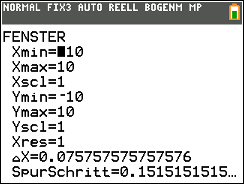
\includegraphics[width=6cm]{Media/GRT/Visualisierung/Fensterbereich_anpassen/fenster}
\end{flushright}
\end{paracol}

\begin{itemize}
	\item[] \texttt{Xscl} Dieser Wert bezeichnet die Schrittlänge auf der X-Achse 
	\item[] \texttt{Ymin} Dieser Wert bezeichnet den minimal zu sehenden Y-Wert auf der Y-Achse
	\item[] \texttt{Ymax} Dieser Wert bezeichnet den maximalen zu sehenden Y-Wert auf der Y-Achse
	\item[] \texttt{Yscl} Dieser Wert bezeichnet die Schrittlänge auf der Y-Achse
\end{itemize} Beim dem Angeben der Werte ist darauf zu achten, dass jegliche negativen Werte nicht mit dem Rechenminus, sonder mit dem Vorzeichenminus angegeben werden. Wurde der Window Bereich eingestellt, kann man im Anschluss mit der Taste \gtr{graph} zu der Ansicht des Koordinatensystems wechseln.
Ist der Graph nicht zu sehen, kann man auch über \gtr{zoom} und anschließend \texttt{zoomStandart} sich wieder die ursprüngliche Einstellung herstellen. 

\subsection{Komplett Reset}
\begin{paracol}{2}
\begin{flushleft}
	Sollte der Fall eines Fehlers auftreten, so ist das maximalinvasivste ein Reset des Taschenrechners, welcher durch die Tagenfolge \gtr{2nd} und \gtr{+}. Anschließend wählt man \texttt{reset} aus.
\end{flushleft}
\switchcolumn
\begin{flushright}
	\includegraphics[width=6cm]{Media/GRT/Visualisierung/komplett_reset/komplett_reset}
\end{flushright}	
\end{paracol}

\subsection{Einsetzen von Werten in eine Funktion}
\begin{paracol}{2}
\begin{flushleft}
	Mit den Tasten \gtr{2nd} und \gtr{trace} lässt sich das Menü zum Berechnen von verschiedenen Funktionsberechnungen aufrufen. Wählt man nun hier \texttt{1} , so kann man einen Wert in eine Funktion einsetzten für die Variable $x$.\\
	Die Dokumentation erfolgt hierbei wie folgt: \\
	\[{value(y_1,Wert)\rightarrow y=Wert}\]
	
\end{flushleft}
\switchcolumn
\begin{flushright}
	\includegraphics[width=6cm]{Media/GRT/Visualisierung/einsetzen_eines_wertes_in_Funktion/einsetzen_eines_wertes_in_Funktion}
\end{flushright}
\end{paracol}
\pagebreak
\subsection{Schnittpunkt ermitteln}

\begin{paracol}{2}
\begin{flushleft}
	Mit den Tasten \gtr{2nd} und \gtr{trace} lässt sich das Menü zum berechnen von verschiedenen Funktionsberechnungen aufrufen. Wählt man\texttt{5}, so kann man den Schnittpunkt von zwei Funktionen berechnen lassen. Hierfür muss man im ersten Schritt die erste Funktion auswähle und anschließend die zweiten und den ungefähren Schnittpunkt der beiden Funktionen.
	\[intersect(y_1,y_2)\rightarrow \quad x=\quad y=\]
	
\end{flushleft}
\switchcolumn
\begin{flushright}
	\includegraphics[width=6cm]{Media/GRT/Visualisierung/Schnittpunkt_ermitteln/Schnittpunkt_ermitteln_1}
	\includegraphics[width=6cm]{Media/GRT/Visualisierung/Schnittpunkt_ermitteln/Schnittpunkt_ermitteln_2}
	\includegraphics[width=6cm]{Media/GRT/Visualisierung/Schnittpunkt_ermitteln/Schnittpunkt_ermitteln_3}
	\includegraphics[width=6cm]{Media/GRT/Visualisierung/Schnittpunkt_ermitteln/Schnittpunkt_ermitteln_4}
\end{flushright}
\end{paracol}

\subsection{Lösen von Gleichungen}
Ist eine Gleichung mit einer Unbekannten in der Grundform $=0$ gegeben, so kann man diese leicht mit dem GTR lösen.

\begin{paracol}{2}
	\begin{flushleft}
	Zuerst erfolgt das Eintragen der Funktion in dem, indem die Funktionen eingetragen werden. Dieses wird aufgerufen, indem man die Taste \gtr{y=} drückt.
		Anschließend drückt man die Taste \gtr{graph}, um sich den Graphen anzeigen zu lassen. 
	\end{flushleft}
\switchcolumn
	\begin{flushright}
	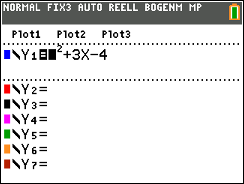
\includegraphics[width= 6cm]{Media/GRT/Visualisierung/loesen_gleichung/loesen_gleichung_1.png}
		\end{flushright}
\end{paracol}


\begin{paracol}{2}
	\begin{flushleft}
	Um nun die Gleichung nach Null aufzulösen, wählt man \gtr{2nd} und \gtr{trace} und wählt Null aus.
		\end{flushleft}
\switchcolumn
	\begin{flushright}
	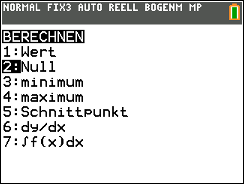
\includegraphics[width= 6cm]{Media/GRT/Visualisierung/loesen_gleichung/loesen_gleichung_2.png}
		\end{flushright}
\end{paracol}

\begin{paracol}{2}
	\begin{flushleft}
	Anschließend müssen die Grenzen bestimmt werden, indem der Taschenrechner die Nullstellen bestimmen soll. Das Wählen der ersten Grenze sollte überhalb der ersten Nullstelle geschehen.
		\end{flushleft}
\switchcolumn
	\begin{flushright}
	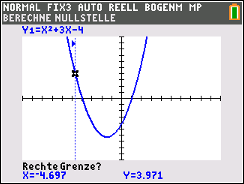
\includegraphics[width= 6cm]{Media/GRT/Visualisierung/loesen_gleichung/loesen_gleichung_3.png}
		\end{flushright}
\end{paracol}

\begin{paracol}{2}
	\begin{flushleft}
	Das Wählen der rechten Grenze geschieht unterhalb der Nullstelle.
		\end{flushleft}
\switchcolumn
	\begin{flushright}
	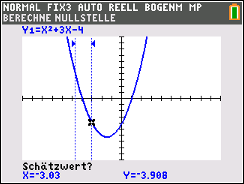
\includegraphics[width= 6cm]{Media/GRT/Visualisierung/loesen_gleichung/loesen_gleichung_4.png}
		\end{flushright}
\end{paracol}

\begin{paracol}{2}
	\begin{flushleft}
	Um schlussendlich die Nullstellen zu bestimmen müssen die Grenzen bestätigt werden. Anschließend zeigt der Taschenrechner die Nullstellen an.
	%TODO Eine Lösung finden die Dokumentation hier zu schreiben, ohne dass ein Fehler auftritt
	%\[(y_1)\rightarrowx=1\quad y=0\]
		\end{flushleft}
\switchcolumn
	\begin{flushright}
	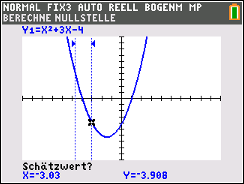
\includegraphics[width= 6cm]{Media/GRT/Visualisierung/loesen_gleichung/loesen_gleichung_4.png}
		\end{flushright}
		
\end{paracol}
\pagebreak

\subsection{Lösen von Gleichungen ohne Graph}
Nicht nur das Lösen nach Null ist möglich mit dem Taschenrechner. Genauso lässt sich eine klassische Gleichung äquvalent umformen mit dem folgenden Vorgehen.

\begin{paracol}{2}
	\begin{flushleft}
	Zunächst navigiert man mit der Taste \gtr{math} auf das \texttt{math} Menu und wählt dort ganz unten die Option \texttt{Numeric Solver} aus. 
	\end{flushleft}	
\switchcolumn
	\begin{flushright}
		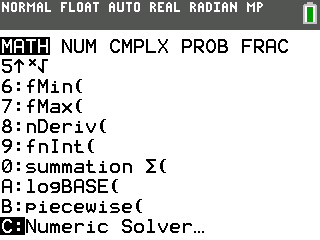
\includegraphics[width=6cm]{Media/GRT/Visualisierung/Gleichung_loesen_aequivalent/Gleichung_loesen_aequivalent_1.png}
	\end{flushright}
\end{paracol}

\begin{paracol}{2}
	\begin{flushleft}
	Nun kann man jeweils die beiden Gleichungen in die Felder \texttt{EQ1} und \texttt{EQ2}
	\end{flushleft}	
\switchcolumn
	\begin{flushright}
		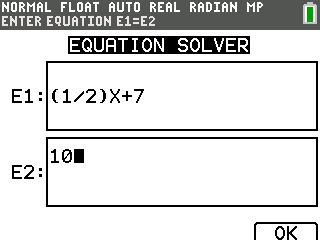
\includegraphics[width=6cm]{Media/GRT/Visualisierung/Gleichung_loesen_aequivalent/Gleichung_loesen_aequivalent_3.png}
	\end{flushright}
\end{paracol}

\begin{paracol}{2}
	\begin{flushleft}
	Abschließend drückt man die Taste unter \texttt{ok}, worauf man in dem folgenden Fenster die Grenzen bestimmen kann. Dies ist nur relevant für Gleichungen, die mehrere Ergebnisse liefern können. 
	\end{flushleft}	
\switchcolumn
	\begin{flushright}
		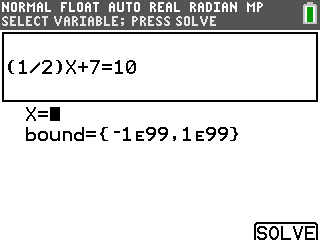
\includegraphics[width=6cm]{Media/GRT/Visualisierung/Gleichung_loesen_aequivalent/Gleichung_loesen_aequivalent_4.png}
	\end{flushright}
\end{paracol}
\begin{paracol}{2}
	\begin{flushleft}
	Abschließend bestätigt man wieder mit der Taste, die unter \texttt{ok} liegt, und erhält ein Ergebnis. 
	\end{flushleft}	
\switchcolumn
	\begin{flushright}
		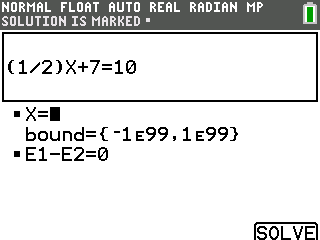
\includegraphics[width=6cm]{Media/GRT/Visualisierung/Gleichung_loesen_aequivalent/Gleichung_loesen_aequivalent_5.png}
	\end{flushright}
\end{paracol}
\subsection{Ableitungsgraph bestimmen}
Auch der Ableitungsgraph lässt sich mit dem Taschenrechner problemlos bestimmen, indem man den \texttt{nDeriv} Befehl anwendet. 
\begin{paracol}{2}
\begin{flushleft}
	Zuerst benötigt man einen bereits eingetragenen Graphen in der Graphenübersicht bei \gtr{y=} und navigiert auf die nächste freie Funktion.
\end{flushleft}
\switchcolumn
\begin{flushright}
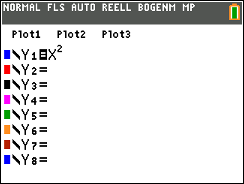
\includegraphics[width=6cm]{Media/GRT/Visualisierung/ableitung_bestimmen/ableitung_bestimmen_1.png}
\end{flushright}
\end{paracol}

\begin{paracol}{2}
\begin{flushleft}
	Nun drückt man die Taste \gtr{math} und wählt aus dem Menu den \texttt{nDeriv} Befehl aus (Herkunft engl. Derivation). Anschließend fügt der Taschenrechner den \texttt{nDrevi} in das Feld der Funktion ein
\end{flushleft}	
\switchcolumn
\begin{flushright}
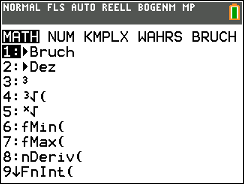
\includegraphics[width=6cm]{Media/GRT/Visualisierung/ableitung_bestimmen/ableitung_bestimmen_2.png}
\end{flushright}
\end{paracol}

\begin{paracol}{2}
\begin{flushleft}
	Hier muss nun die umpunkteten Feldern ein Wert eingetragen werden. Der Bruch wird wie folgt definiert $\frac{d}{dx}$. In die Klammer wird die Funktion deren Ableitung gewünscht ist eingetragen mit deer Taste \gtr{alpha} und \gtr{trace} drauf öffnet sich Menu aus Funktionen, die dort eingesetzt werden können. Zuletzt wird in dem hintersten Feld erneut $x$ eingetragen. Drückt man nun erneut \gtr{graph}, so erhält man den Ableitungsgraph der Funktion.
	\end{flushleft}	
\switchcolumn
\begin{flushright}
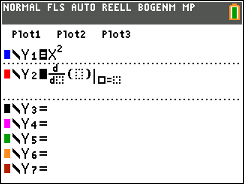
\includegraphics[width=6cm]{Media/GRT/Visualisierung/ableitung_bestimmen/ableitung_bestimmen_3.png}
\end{flushright}
\end{paracol}
\pagebreak
\subsection{Integrale berechnen}
Ähnlich wie bei der Ableitung ist es möglich das Integral graphisch zu bestimmen. Der GTR kann hierbei auch rechnerisch vorgehen. 

\begin{paracol}{2}
\begin{flushleft}
	Um ein Integral mit dem GTR rechnerisch zu bestimmen, muss zunächst \gtr{2nd} und \gtr{trace} gedrückt werden. Anschließend navigiert man zu der Option 7:$\int f(x)dx$
\end{flushleft}	
\switchcolumn
\begin{flushright}
	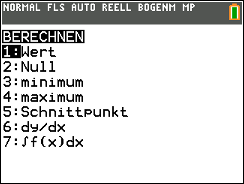
\includegraphics[width=6cm]{Media/GRT/Visualisierung/Integrale_berechnen/Integrale_berechnen_1.png}
\end{flushright}
\end{paracol}

\begin{paracol}{2}
\begin{flushleft}
	Anschließend kann die linke Grenze des Integrals graphisch gewählt werden.
\end{flushleft}	
\switchcolumn
\begin{flushright}
	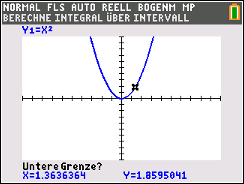
\includegraphics[width=6cm]{Media/GRT/Visualisierung/Integrale_berechnen/Integrale_berechnen_2.png}
\end{flushright}
\end{paracol}

\begin{paracol}{2}
\begin{flushleft}
	Nachdem die linke Intervallgrenze gesetzt wurde, muss nun die rechte gewählt werden. Dies funktioniert gleich wie bei der linken.
\end{flushleft}	
\switchcolumn
\begin{flushright}
	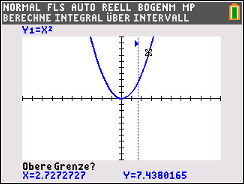
\includegraphics[width=6cm]{Media/GRT/Visualisierung/Integrale_berechnen/Integrale_berechnen_3.png}
\end{flushright}
\end{paracol}

\begin{paracol}{2}
\begin{flushleft}
	Nachdem mit der Enter Taste bestätigt wurde, verfärbt sich der gewählte Intervall und zeigt den Flächeninhalt in dem jeweiligen Intervall an. 
\end{flushleft}
\switchcolumn
\begin{flushright}
	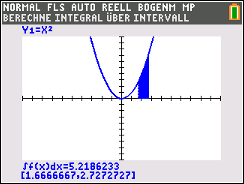
\includegraphics[width=6cm]{Media/GRT/Visualisierung/Integrale_berechnen/Integrale_berechnen_4.png}
\end{flushright}
\end{paracol}
\pagebreak
\subsection{Unbekannte Intervallgrenzen eintragen}
Um eine bekannten Flächeninhalt mit einer unbekannten Intervallgrenze zu berechnen, geht man wie folgt vor.
\begin{paracol}{2}
\begin{flushleft}
	Eintragen der Ausgangsfunktion in das Funktionsmenü bei \gtr{y=}
\end{flushleft}	
\switchcolumn
\begin{flushright}
\begin{figure}
	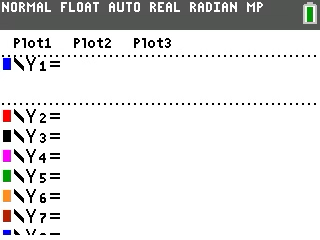
\includegraphics[width=6cm]{Media/GRT/Visualisierung/unbekannte_intervallgrenze/unbekannte_intervallgrenze_1.gif}
	\caption{\link{https://youtu.be/it9pl_ZB9wc}{Visualisierung}}
\end{figure}
\end{flushright}
\end{paracol}
Anschließend muss nun das Integral eingetragen werden. Hierfür drückt man zunächst auf die Taste \gtr{math}und wählt anschließend die Option \texttt{fnInt()} aus. Nun müssen die Integralgrenzen eingefügt werden. Die erste bekannte Intervallgrenze wird unten eingefügt, während die unbekannte mit $x$ ersetzt wird. Hiernach muss die Funktion eingetragen werden, so wie die Variable, nach der hier aufgelöst wird. Abschließend kann die Taste \gtr{graph} gedrückt werden. Auf dem Graphen Fenster ist nun die Stammfunktion zu sehen.
\pagebreak
\subsection{Berechnung nicht-orientierter Flächen}
Um anstatt mit orientierten Flächen mit dem reinen Flächeninhalt zu rechnen, muss mit dem Betrag gerechnet werden.
\begin{paracol}{2}
\begin{flushleft}
	Zunächst müssen die Nullstellen mit dem Befehl \texttt{zero} ermittelt werden. Hierfür geht man auf \gtr{2nd} und \gtr{trace}, wählt dort \texttt{zero} aus und gibt nun Rechts und Links die Grenzen der Nullstelle an. Abschließend drückt man Enter und erhält die X-Koordiante. Dieser Vorgang ist Abhängig von der Anzahl der Nullstellen und muss ggf. mehr als zwei mal wiederholt werden. 
\end{flushleft}	
\switchcolumn
\begin{flushright}
	\begin{figure}
		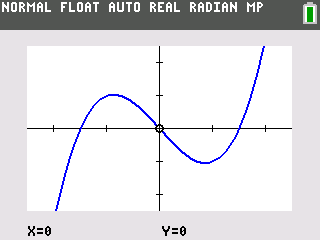
\includegraphics[width=6cm]{Media/GRT/Visualisierung/berechnung_nichtOrientierter_Flacheninhalt/berechnung_nichtOrientierter_Flacheninhalt_1.png}
		\caption{\link{https://youtu.be/MD6kzV_FIQc}{Visualisierung}}

	\end{figure}
	\end{flushright}
\end{paracol}
Anschließend muss nun der Flächeninhalt zwischen dem Graphen und der X-Achse berechnet werden mithilfe der Betragsstriche. Hierfür benutzt man die im vorherigen Schritt berechneten Nullstellen als Intervallgrenzen und berechnet den jeweiligen Flächeninhalt. Diese werden anschließend addiert, worauf man den gesamten Flächeninhalt des Graphen in einem Intervall hat. 
	Die Druchführung der Addition darf nicht im Bereich der Funktion durchgeführt werden, da hierbei sich nur einen Gleichung ergibt, welche als lineare dargestellt wird. Um nun ein Integral einzutragen verwendet man \gtr{math} und wählt die Option \texttt{fnInt()} an. Anschließend kann man die Intervallgrenzen(berechneten Nullstellen) eintragen. Um nun denBetrag einer Funktion zu verwenden, muss man auf \gtr{math} drücken und dort mit den Pfeiltasten auf die Kategorie \texttt{NUM} navigieren. Dort wählt man \texttt{abs()} aus und bestätigt mit Enter. 
\pagebreak
\subsection{Flächeninhalt zwischen zwei Funktionen berechnen}
Bei berechnen von einem Flächeninhalt zwischen zwei Funktionen stellt sich ein ähnliches Problem Problem heraus wie bei berechnen des Flächeninhalts mit der X-Achse.
\begin{paracol}{2}
	\begin{flushleft}
	Um den Flächeninhalt mit dem GTR zu berechnen, bildet man zunächst die Differenzenfunktion, indem man sich bei Funktionen in der Funktionsübersicht einträgt und anschließend eine weitere definiert. Diese Funktion subtrahiert die beide vorherigen Funktionen von einandern. 
	\end{flushleft}
\switchcolumn
	\begin{flushright}
		\begin{figure}
			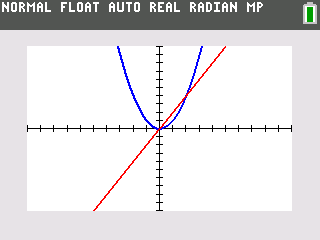
\includegraphics[width=6cm]{Media/GRT/Visualisierung/Flaecheninhalt_zwischen_zwei_Funktionen_berechnen/Flaecheninhalt_zwischen_zwei_Funktionen_berechnen.png}
		\caption{\link{https://youtu.be/y-6UFVmVIOE}{Visualsisierung}}
		\end{figure}
	\end{flushright}
\end{paracol}
\pagebreak
\subsection{Regression}
Die Regression ist ein Verfahren, bei dem Zusammenhänge zwischen Abhängigkeiten einer oder mehrere Variablen analysiert werden. Beim GTR gibt es verschiedene Arten, die für verschiedenen Graphen sind. Diese Arten sind spezifisch für spezifische Graphen gedacht, weswegen das wählen dieser sorgfältig erfolgen sollte. 

\begin{paracol}{2}
\begin{flushleft}
	Um mithilfe von Regression eine Funktionsgleichung zu bestimmen geht man über \gtr{stat} in das \texttt{STAT}-Menu.
\end{flushleft}	
\switchcolumn
\begin{flushright}
	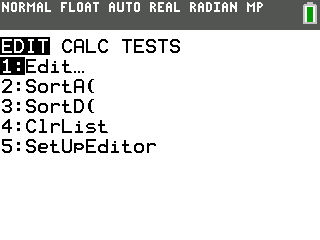
\includegraphics[width=6cm]{Media/GRT/Visualisierung/Regression/Regression_1.png}
\end{flushright}
\end{paracol}

\begin{paracol}{2}
	\begin{flushleft}
	Anschließend wählt man Edit aus und kommt in die Listenansicht. In dieser müssen nun mindestens zwei verschiedene Punkte eingetragen werden. In der ersten Spalte befinden sich hierbei die X-Wert und in der zweiten die Y-Werte. 
	\end{flushleft}	
\switchcolumn
	\begin{flushright}
		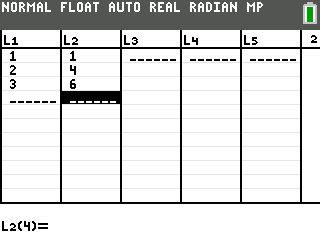
\includegraphics[width=6cm]{Media/GRT/Visualisierung/Regression/Regression_5.png}
	\end{flushright}
\end{paracol}

\begin{paracol}{2}
	\begin{flushleft}
	Sind die Werte eingetragen, so drückt man erneut \gtr{stat} und navigiert mit den Pfeiltaste in das \texttt{Calc} Menu. Dort wählt man\texttt{QuadReg} aus und bestätigt.
	\end{flushleft}	
\switchcolumn
	\begin{flushright}
		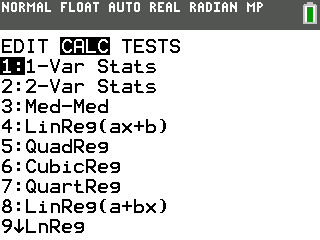
\includegraphics[width=6cm]{Media/GRT/Visualisierung/Regression/Regression_3.png}
	\end{flushright}
\end{paracol}

\begin{paracol}{2}
	\begin{flushleft}
	Bestätigt man erneut kommt man in eine Bestätigungsansicht, wo die jeweiligen Listen erneut ausgewählt werden müssen. Bestätigt man dies, so erhalt man 
	\begin{center}
			\texttt{LinReg}\\
			\end{center}
			\texttt{y=ax+c}\\
			\texttt{a=-05}\\
			\texttt{c=3}
	\end{flushleft}	
\switchcolumn
	\begin{flushright}
		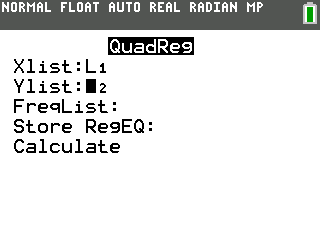
\includegraphics[width=6cm]{Media/GRT/Visualisierung/Regression/Regression_4.png}
		
	\end{flushright}
\end{paracol}
\pagebreak












